\documentclass{article}
\usepackage[margin=1.5cm]{geometry}
\usepackage{amsmath}
\usepackage{graphicx}
\usepackage{booktabs}
\usepackage{xeCJK}
\usepackage{ragged2e}
\usepackage{paracol}
\setlength{\emergencystretch}{3em}
\begin{document}
\sloppy

\noindent\hfill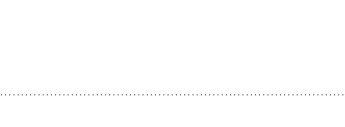
\includegraphics[height=1.8em]{assets/figure_header_logo.png}\par\noindent\hrule\vspace{4pt}
\begin{paracol}{3}
\RaggedRight

财经智库FINANCIAL MINDS

\switchcolumn
\RaggedRight

\subsection*{参考文献}

\switchcolumn
\RaggedRight

(责任编辑：雪宁)

\end{paracol}


出现非常明显的聚束，如果我们能够计算出这种聚束的幅度，就能够用来估计个税税率对劳动者产生的负向激励作用。


范子英、李欣：“部长的政治关联效应与财政转移支付分配”，《经济研究》2014年第6期。刘甲炎、范子英：“中国房产税试点的效果评估：基于合成控制法的研究”，《世界经济》2013年第11期。Angrist, J.D. and Pischke, Jörn-Steffen, 2009, Mostly Harmless Econometrics,Princeton University Press.Chen, Y.Y., Ebenstein, A., Greenstone, M. and H.B., Li, 2013, Evidenceon the Impact of Sustained Exposure to Air Pollution on Life Expectancy from China'sHuai River Policy, Proceedings of the National Academy of Sciences, 110 ( 32 ) :12936-12941.

\end{document}
